\vzmstitle{СТАБИЛИЗАЦИЯ И УПРАВЛЕНИЕ СИСТЕМАМИ С ГИСТЕРЕЗИСНЫМИ НЕЛИНЕЙНОСТЯМИ}
\vzmsauthor{Решетова}{О.\,О.}
\vzmsauthor{Семенов}{М.\,Е.}
\vzmsauthor{Мелешенко}{П.\,А.}
\vzmsauthor{Соловьев}{А.\,М.}
\vzmsauthor{Борзунов}{С.\,В.}
\vzmsauthor{Толкачев}{А.\,В.}
\vzmsinfo{Воронеж; {\it tribunskih1993@mail.ru}}
\vzmscaption

\textbf{Введение}\\
Моделирование прикладных задач в различных предметных областях, таких как: системы автоматического регулирования, теория твердого тела, описании различных экономических и биологических процессах, связано с изучением колебательных явлений. Задачи стабилизации и управления подобными системами, с практической точки зрения, являются одними из основных. Зачастую, эти задачи сводятся к системам дифференциальных уравнений, содержащим как функциональные нелинейности, так и нелинейности гистерезисной природы [1]. В настоящей работе проводится исследование ряда динамических систем с гистерезисными нелинейностям.\\

\textbf{Гистерезисный демпфер основанный на модели Боука-~Вена}\\
Рассмотрим механическую систему, находящуюся под действием вынуждающей периодической силы при наличии демпфирующего звена [2] (рис. 1). Механическая система состоит из цилиндра массой $M$, груза массой $m$, пружины с жесткостью $k$ и демпфирующего звена $D$, двигающийся без трения в горизонтальной плоскости. К цилиндру приложена вынуждающая сила $f(t)$ изменяющаяся по гармоническому закону.\\
\begin{figure}
\center{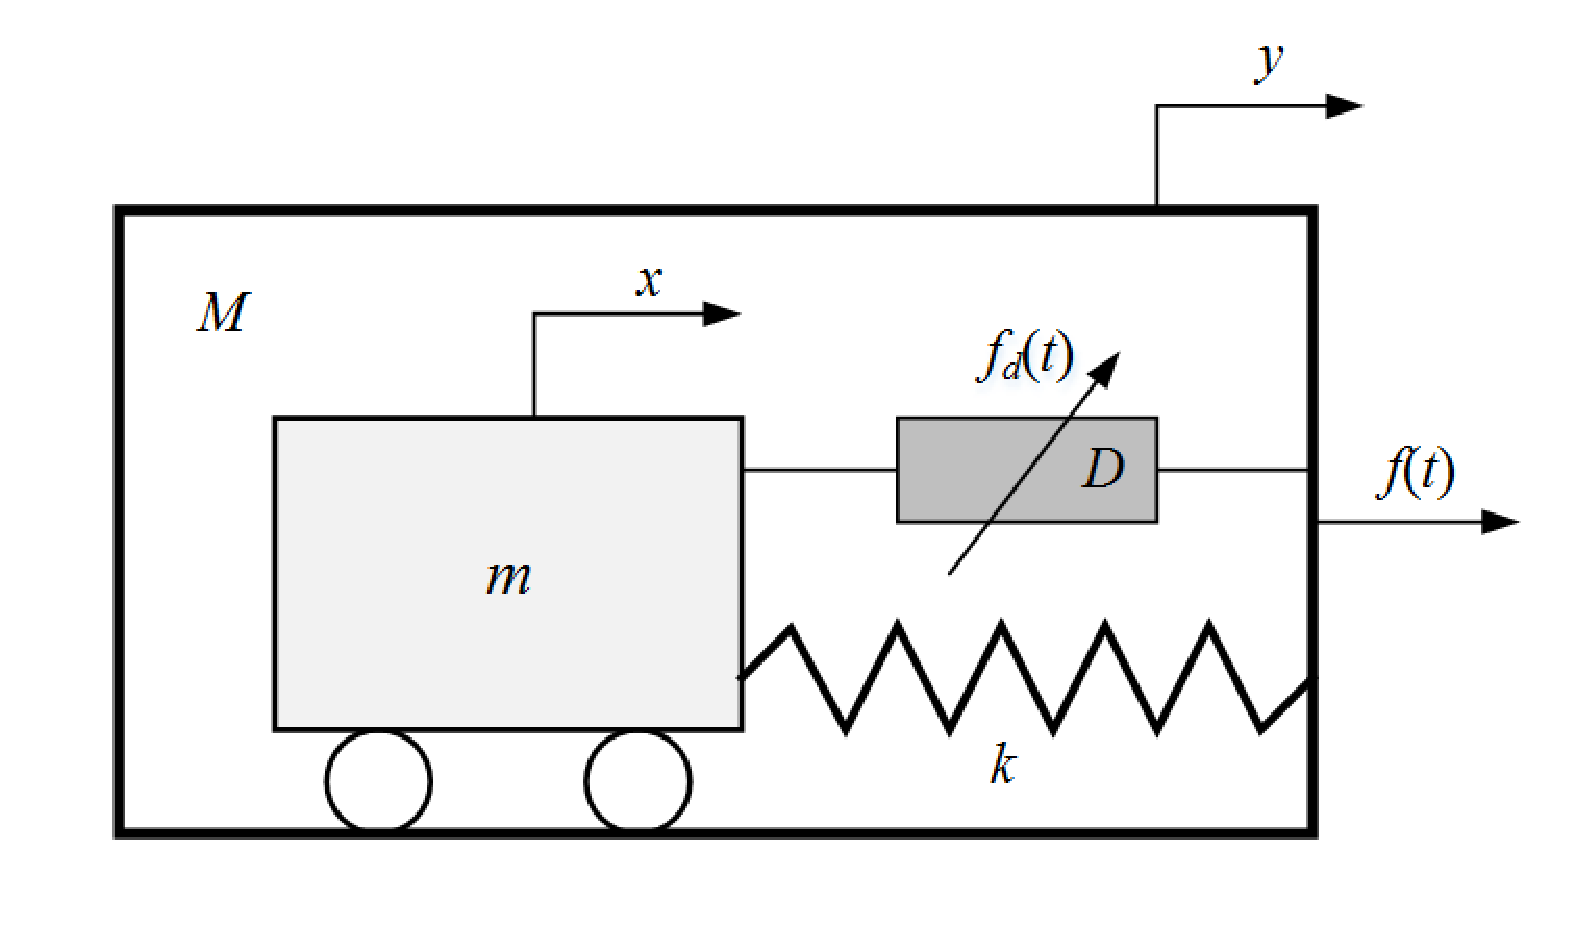
\includegraphics[width=0.5\linewidth]{im1.eps}}
\hfill
\caption*{Рис.1. Исследуемая механическая система }
\label{ris:correlationsignals}
\end{figure}
Пусть закон изменения силы $f(t)$, приложенной к цилиндру $M$:\\
$$f(t)=Y\omega^{2}\sin(\omega t)\eqno (1)$$
где $Y$ – амплитуда, $\omega$ – частота воздействия.\\
Рассмотрим гистерезисный демпфер на основе феноменологической модели Боука-Вена[3]. Демпфирующая сила может быть представлена как:\\
$$\ddot{u}+\xi(k_{b}g+ku)=A\Omega^{2}\sin(\Omega t),\xi=\frac{1}{\omega_{0}\mu},$$
$$\dot{g}_{\tau}=\dot{u}_{\tau}\left(B-(\beta sign[g\dot{u}_{\tau}]+\gamma)|g|^{p}\right). \eqno (2)$$\\
где $\Omega$,$\mu$, $A$, $\tau$, $\omega_{0}$, $\xi$ -~ безразмерные величины. Проведем сравнительный анализ вязкого и гистерезисного демпферов. Сравнение указанных типов демпфирующих элементов наиболее репрезентативно может быть представлено в терминах передаточных функций, отражающих эффективность использования рассматриваемого демпфера в области резонанса системы и за ее пределами.\\
Передаточная функция силы:\\
$$T_{ff}=\frac{1}{Y\omega^{2}}max\left|m\omega_{0}^{2}\frac{d^{2}x}{d\tau^{2}}\right|\eqno (3)$$\\
Передаточная функция «перемещение-сила»:\\
$$T_{fd}=\frac{max |x(\tau)|}{Y\omega^{2}}\eqno (4)$$\\
\begin{figure}
\center{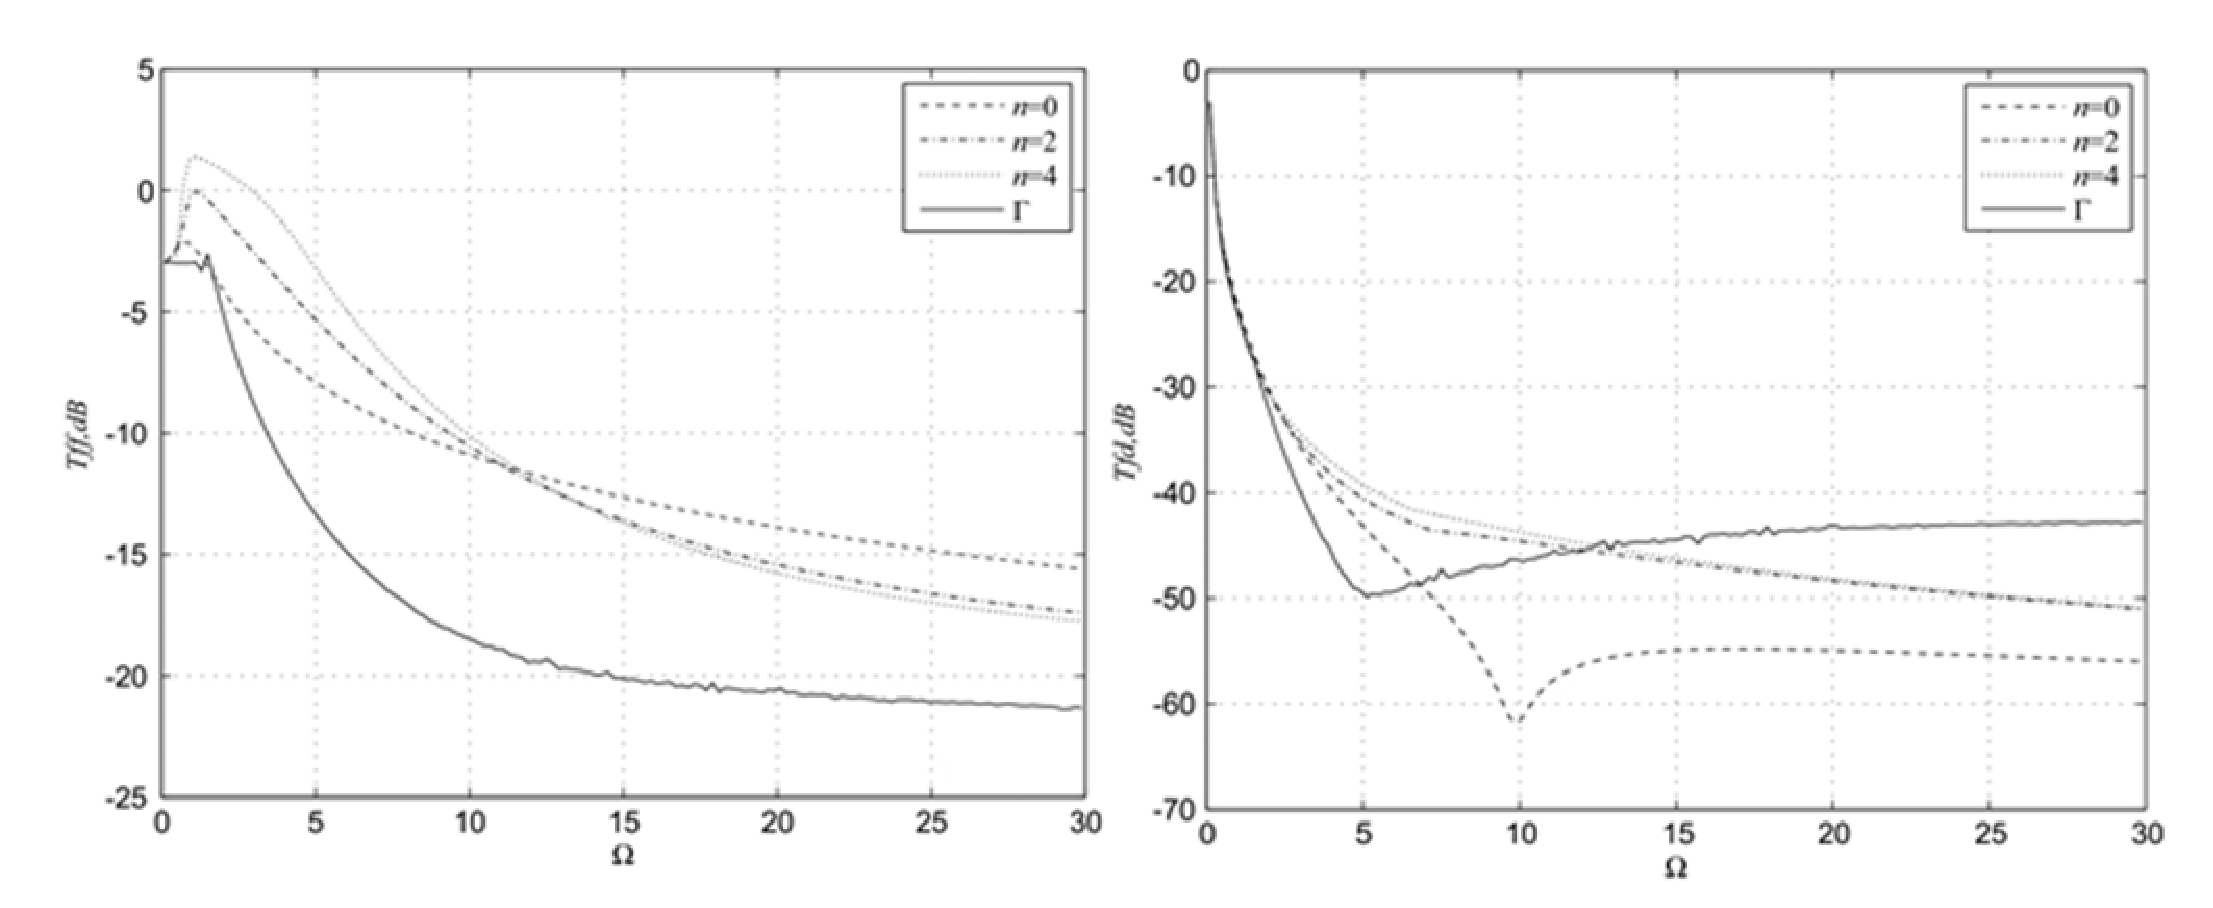
\includegraphics[width=0.8\linewidth]{im2.eps}}
\hfill
\caption*{Рис.2. Передаточные функции силы (слева) и «перемещение-сила» (справа) для гистерезисного (Г), линейного вязкого $(n=0)$ и нелинейного вязкого $(n>0)$ демпферов }
\label{ris:correlationsignals}
\end{figure}
Как видно из результатов моделирования (рис.2), в случае использования гистерезисного демпфера на основе феноменологической модели Боука- Вена, возможно добиться высокой эффективности демпфирования как в области резонанса, так и за ее пределами, по сравнению с использованием линейного или нелинейного вязкого демпферов.\\

\textbf{Динамика гармонического осциллятора с гистерезисным внешним воздействием}\\
Рассмотрим систему, динамика которой описывается задачей Коши с начальными условиями $x(0)=x_{0},\dot{x}(0)=x_{1}$.\\
$$\ddot{x}+\omega^{2}x=R[\alpha,\beta, \omega_{0}],\eqno (5)$$\\
где $R[\alpha,\beta,\omega_{0}]$ -~оператор неидеального реле с инверсией пороговых чисел.\\
\textbf{Теорема~1.} {\it Пусть $x_{0}\notin [\alpha,\beta]$.  Тогда отвечающее ему решение не ограничено.}\\
Иными словами, если начальное значение таково, что гистерезисное звено, «срабатывает», то решение ему соответствующее не ограничено [4].\\
\begin{figure}
\center{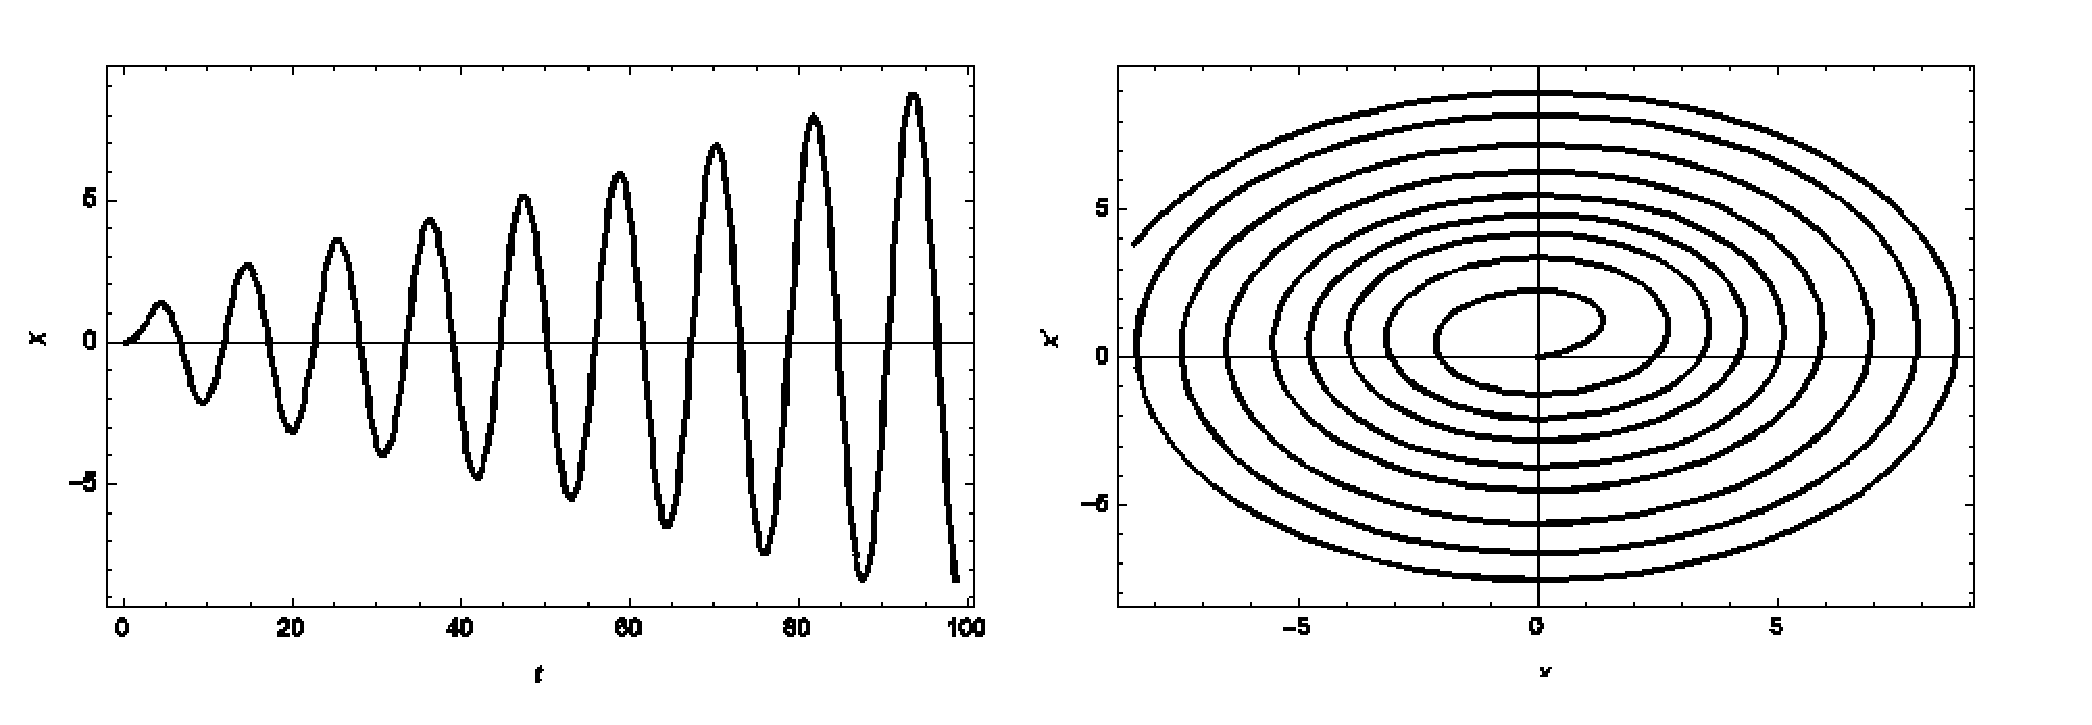
\includegraphics[width=0.8\linewidth]{im3.eps}}
\hfill
\caption*{Рис.3. Решение и фазовый портрет уравнения (5) с заданными начальными условиями }
\label{ris:correlationsignals}
\end{figure}
\textbf{Замечание~1.} {\it Очевидно, что решение будет осциллировать и при этом скорость роста амплитуды будет пропорциональна  $\sqrt{t}$.}\\
\textbf{Замечание~2.} {\it Очевидно, что теорема остается верной и для других гистерезисных нелинейностей. Единственное требование к ним заключается в положительной площади петли.}\\

\textbf{Динамика осциллятора ван дер Поля под воздействием гистерезисного управления }\\
Система уравнений (6) описывает осциллятора ван дер Поля, под воздействием периодической внешней силы, а также гистерезисного управления формализованного при помощи модели Боука-Вена.
$$\ddot{x}-(\lambda-x^{2})\dot{x}+\omega^{2}_{0} x  =  A \cos [\omega t]+\Phi_{BW}(x,t),$$
$$\Phi_{BW}(x,t) =  \alpha x(t)+(1-\alpha)Dz(t), \eqno (6)$$
$$\dot{z}(t) =  A_{1}\dot{x}(t)-\beta|\dot{x}(t)||z(t)|^{n-1}z(t)-\gamma \dot{x}(t)|z(t)|^{n}.$$
Начальные и граничные условия определены аналогично с системой (5).\\
Проведя сравнительный анализ результатов численного моделирования системы (6) известными результатами для уравнения ван дер Поля без учета гистерезисного блока, было установлено, что включение гистерезисного звена приводит к диссипации энергии и, как следствие, к изменению динамических характеристик рассматриваемой системы. Ниже приведены биффуркационные диаграммы, отражающие существенное различие в поведении систем. Подсчет спектра показателей Ляпунова, с использованием стандартного подхода основанного на алгоритме Вольфа, подтвердил полученные результаты.\\
\begin{figure}
\center{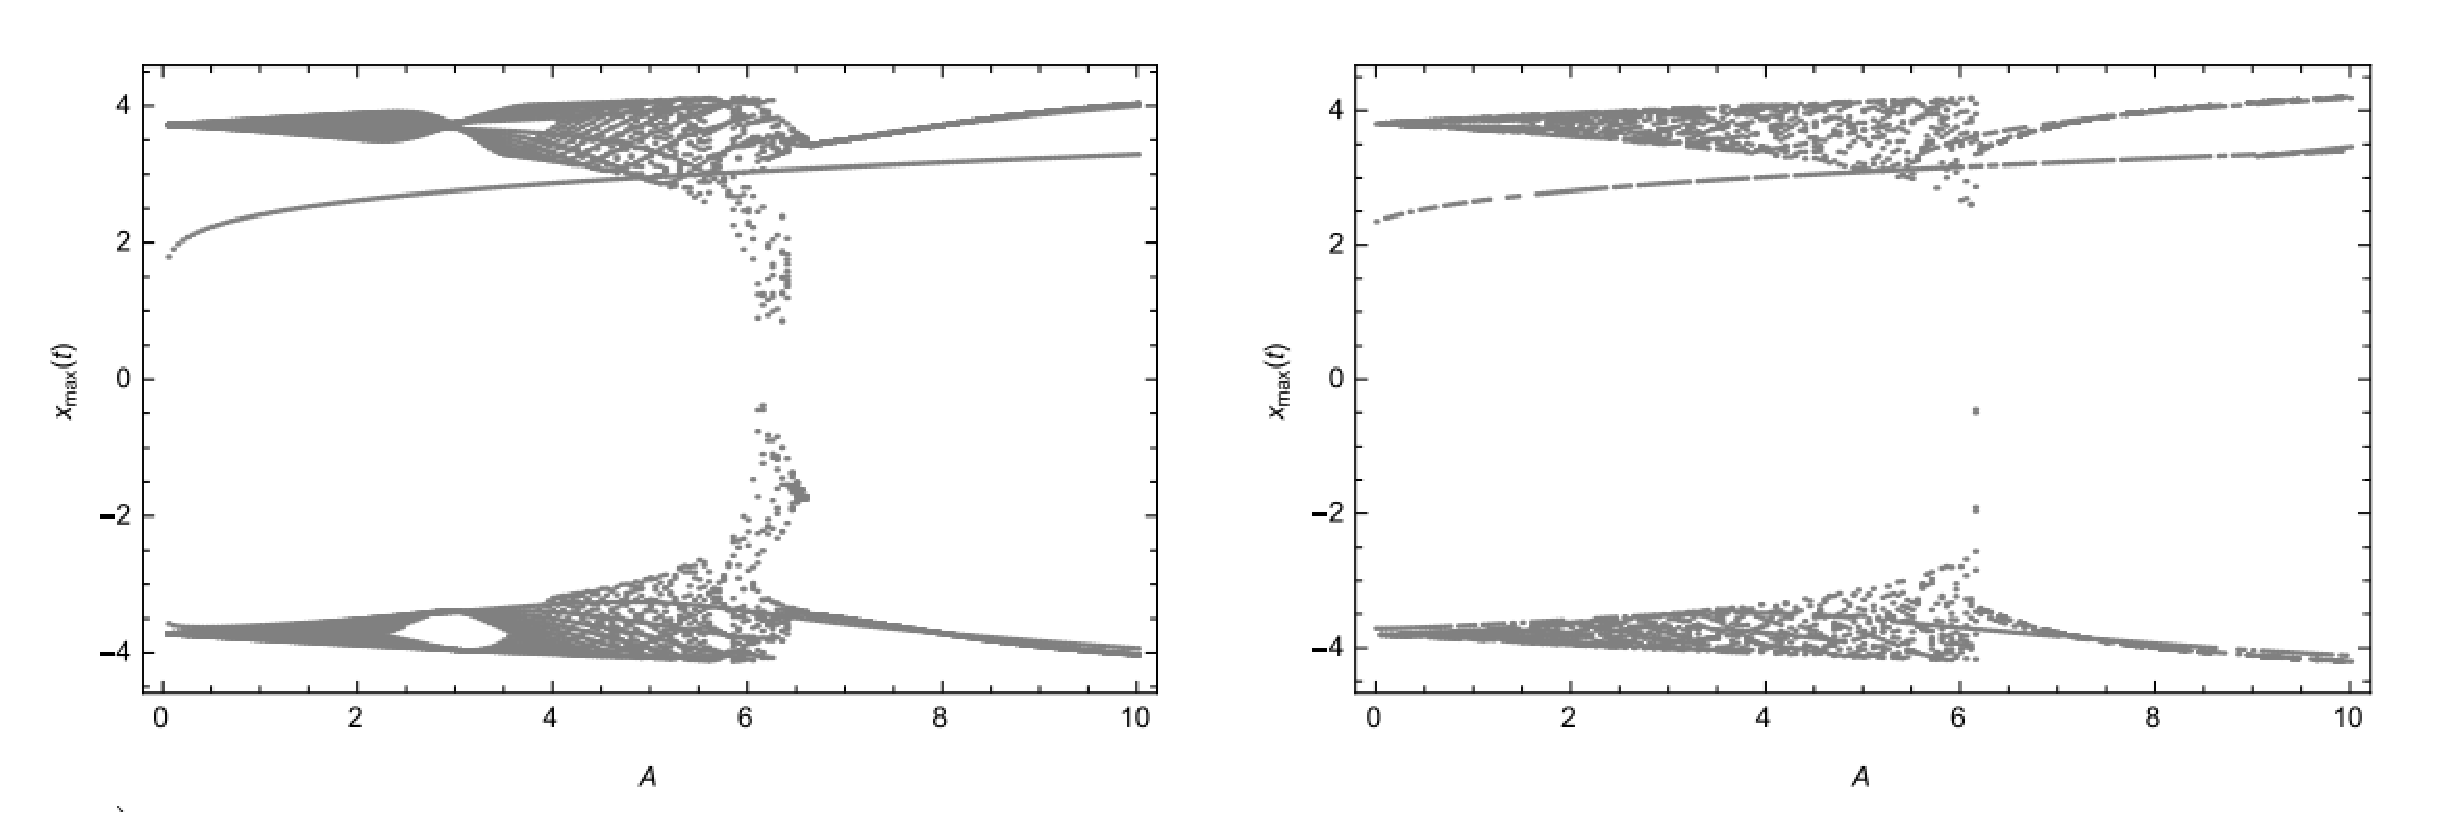
\includegraphics[width=0.8\linewidth]{im4.eps}}
\hfill
\caption*{Рис.4. Бифуркационные диаграммы в зависимости от амплитуды внешнего воздействия для системы без гистерезисного блока и системы (6) при значении параметров $\lambda=3.4$, $\omega^{2}_{0}=\pi$, $A=2\pi$, $\omega=0.7$ }
\label{ris:correlationsignals}
\end{figure}

\textbf{Заключение}\\
В результате исследования колебательной системы с гистерезисным звеном удалось показать, что гистерезисный вибрационный демпфер основанный на феноменологической модели Боука-Вена имеет ряд важных преимуществ по сравнению с демпферами, построенными на основе вязкого трения.\\
Также в работе были исследованы резонансные свойства системы, в которой рассеивание энергии обусловлено наличием гистерезисного звена, а внешнее воздействие имеет резонансную частоту.\\
В ходе работы была установлена возможность управления хаотической динамикой осциллятора ван дер Поля с периодическим возмущением. На основе анализа численных результатов бифуркационных диаграмм и соответствующей динамики показателей Ляпунова установлена эффективность регуляризирующей роли гистерезисного звена.\\

\textbf{Благодарность}\\
Работа выполнена при финансовой поддержке РФФИ (проект 19-08-00158);\\
Работа М.Е. Семенова и П.А. Мелешенко в части «Динамика системы ван дер Поля») поддержана РНФ (грант 19-11-0197).

% Оформление списка литературы
\litlist
1. {\it Семенов М.Е.} Динамика демпфирующего устройства на основе материала Ишлинского ~/ М.Е. Семенов, М. Г. Матвеев, П.А. Мелешенко, А. М. Соловьёв~// Мехатроника, автоматизация, управление. ~---2019. ~--- №~20(2). ~--- C.~106--113.

2. {\it Semenov M. E.} Nonlinear Damping: From Viscous to Hysteretic Dampers ~/M. E. Semenov, A. M. Solovyov, P. A. Meleshenko et al. ~// Proceedings in Physics. ~---2018. ~---Vol.~199.

3. {\it Ikhouane F.} On the Hysteretic Bouc-Wen Model ~/ F. Ikhouane, J. Rodellar ~// Nonlinear Dynamics. ~--- 2005. ~--- Vol.~42. ~--- P.~63--78.

4. {\it Solovyov A. M.} Hysteretic nonlinearity and unbounded solutions in oscillating systems ~/ A. M. Solovyov, M. E. Semenov, P. A. Meleshenko et al. ~// Procedia Engineering. ~---2017. ~--- Vol.~201. ~--- P.~578--583.
